\documentclass{article}

\usepackage[preprint]{icml2026}
\usepackage{microtype}
\usepackage{booktabs}
\usepackage{amsmath,amssymb}
\usepackage{graphicx}
\usepackage{multirow}
\usepackage{xcolor}
\usepackage{url}

\icmltitlerunning{recovery}

\begin{document}

\twocolumn[
\icmltitle{Does Context Order Leave a Lasting Trace?\\
A Recovery-Based Study of Sequence-Length Curricula}

\begin{icmlauthorlist}
\icmlauthor{Anqi Zu}{oxford}
\end{icmlauthorlist}
\icmlaffiliation{oxford}{University of Oxford}
\icmlcorrespondingauthor{Anqi Zu}{angela.zoo@foxmail.com}
\icmlkeywords{training dynamics, curriculum learning, sequence length, controlled experiments}

\vskip 0.3in
]

\printAffiliationsAndNotice{}

\begin{abstract}
Sequence-length curricula change both the order of training contexts and the context seen immediately before evaluation, making terminal comparisons difficult to interpret. We study this ambiguity in a preregistered, paired experiment on a 4.8M-parameter character-level Transformer: ascending and descending schedules receive the same four context-length blocks, token throughput, optimizer policy, and data draws, followed by 500 identical long-context recovery updates. Before recovery, descending training is worse at the 256-token evaluation horizon by $0.7570$ bits per character (BPC; 95\% $t$ interval $[0.3290,1.1851]$, three of three seeds positive); after recovery the contrast reverses to $-0.0485$ BPC ($[-0.1491,0.0521]$). Process measurements show that most of the long-horizon gap disappears within 50 recovery steps, while shorter-horizon contrasts were already small before recovery. Thus the large terminal deficit is not evidence of a lasting positive path-dependent penalty, but the reversed residual lies outside our preregistered practical-removal band and remains unresolved. The study illustrates a compact recovery-test design---paired data, common recovery, multi-horizon evaluation, and dense transition-local measurement---for separating transient terminal-context alignment from persistent training-order effects.
\end{abstract}

\section{Introduction}

Curricula alter what a model sees and \emph{when} it sees it. This is precisely their appeal, but it also complicates causal interpretation: two schedules that contain the same training conditions can end in different states simply because their final blocks differ. A terminal evaluation may therefore conflate a persistent effect of training order with a transient match between the most recent training context and the evaluation context.

Sequence length makes this problem unusually concrete. Length schedules are used to reduce early training cost or improve optimization stability \citep{press2021shortformer,li2022slw,pouransari2024dataset}. Yet an ascending schedule ends at long context and a descending schedule ends at short context. If both are evaluated only at long context, an observed gap need not reveal whether the historical ordering left a durable trace.

We ask: \emph{after matched exposure to the same context lengths, does their temporal order leave a persistent performance difference under a common long-context recovery stage?} We compare ascending ($32{\rightarrow}64{\rightarrow}128{\rightarrow}256$) and descending ($256{\rightarrow}128{\rightarrow}64{\rightarrow}32$) schedules using paired initialization and context-specific data manifests. Both then receive 500 identical updates at context length 256. We measure fixed validation targets at four evaluation horizons, using a small process panel at 17 checkpoints and a larger anchor panel at the preregistered endpoints.

The large pre-recovery long-context deficit reverses under common recovery: the descending-minus-ascending contrast changes from $+0.7570$ to $-0.0485$ BPC. The process trajectory falls by over 90\% in ten steps and crosses zero by 50 steps. Crucially, the pre-recovery gap is concentrated at the 256-token evaluation horizon rather than reflecting uniform degradation. These observations are consistent with a strong terminal-context-sensitive component. They do not identify a unique mechanism, and three seeds do not resolve the smaller negative residual.

Our contributions are:
\begin{itemize}
    \item an empirical result showing that a large terminal long-context deficit does not survive matched long-context recovery in this setting;
    \item a recovery-test design that combines a preregistered paired endpoint with transition-local trajectories and multiple evaluation horizons; and
    \item a transparent account of an outcome that contradicts the simplest preregistered expectation: the original gap reverses sign but does not enter the practical-removal region.
\end{itemize}

\section{Related Work}

\paragraph{Curricula and data order.}
Curriculum learning organizes examples by difficulty or competence \citep{bengio2009curriculum,zhou2021curriculum}. In language modeling, order can interact with initialization, optimization, and data presentation; run-to-run variation from data order is itself consequential \citep{dodge2020finetuning}. Our experiment targets a narrower estimand: the total effect of permuting four length blocks under one fixed training policy.

\paragraph{Sequence-length schedules.}
Training first on shorter sequences can reduce compute or stabilize early optimization. Shortformer separates early short-context training from later long-context training \citep{press2021shortformer}; sequence-length warmup gradually increases length to address stability and efficiency \citep{li2022slw}; dataset decomposition studies length and difficulty schedules at larger scale \citep{pouransari2024dataset}. These works motivate length as a meaningful training variable. We instead focus on an identification problem: whether a terminal difference survives when schedules are placed under an identical post-treatment task.

\paragraph{Dynamics and uncertainty.}
Endpoint-only evaluation can conceal qualitatively different learning trajectories, as illustrated by delayed generalization and other non-monotone dynamics \citep{power2022grokking}. Small-sample comparisons also demand raw-run reporting and effect-size uncertainty rather than reliance on thresholded significance \citep{agarwal2021precipice,ho2019estimation}. We therefore expose paired seed trajectories and Student-$t$ intervals, while treating near-zero claims as unresolved rather than equivalent.

\section{Recovery Tests for Context-Order Effects}

Let $s\in\{\mathrm{asc},\mathrm{desc}\}$ denote a schedule, $h$ an evaluation horizon, and $k$ the number of common recovery updates after the scheduled phase. Define the paired contrast
\begin{equation}
\Delta_h(k)=\mathrm{BPC}_{\mathrm{desc},h}(2000+k)-
\mathrm{BPC}_{\mathrm{asc},h}(2000+k).
\end{equation}
Positive values mean descending is worse. The preregistered primary estimand uses the 32-sequence anchor panel at $h=256$ and $k\in\{0,500\}$, denoted $\Delta^A_{256}(k)$. Absolute recovery is
\begin{equation}
G=\Delta^A_{256}(0)-\Delta^A_{256}(500),
\end{equation}
and, when the initial gap is at least $0.02$ BPC, the descriptive recovery ratio is
\begin{equation}
R=\frac{\Delta^A_{256}(500)}{\Delta^A_{256}(0)}.
\end{equation}

The logic is counterfactual rather than mechanistic. A substantial same-sign residual after common recovery is compatible with persistent path dependence. Rapid decay concentrated at the horizon matching the terminal training block is compatible with a transient terminal-context-sensitive component. Neither pattern uniquely identifies optimizer state, representation change, or memorization. To track horizon dependence we additionally define, on the 16-sequence process panel,
\begin{equation}
A^P(k)=\Delta^P_{256}(k)-\Delta^P_{32}(k).
\end{equation}

Before training, we registered $R<0.25$ as evidence that at least 75\% of the original positive gap was removed. This ratio could not override the absolute endpoint rule: practical removal required $|\operatorname{mean}\Delta^A_{256}(500)|\leq0.02$ BPC. A positive residual above $0.03$ BPC in all seeds, together with a plateau, was required before launching a mechanism study. These are project-level decision thresholds, not universal scientific constants.

\section{Experimental Design}

\subsection{Controlled comparison}

We train a 4.8M-parameter, six-layer, eight-head, character-level Transformer with rotary position embeddings \citep{vaswani2017attention,su2021roformer} on Tiny Shakespeare. The two primary schedules each contain four 500-step blocks. An exploratory nonmonotonic schedule ($64{\rightarrow}256{\rightarrow}32{\rightarrow}128$) is excluded from primary inference and reported only in Appendix~\ref{app:nonmono}.

All arms receive 4,096 target tokens per optimizer update by setting batch size to $4096/h$. We hold architecture, tokenizer, split, number of updates, global learning-rate schedule, AdamW configuration \citep{loshchilov2019adamw}, gradient clipping, and evaluation targets fixed. Within each seed, arms share initial weights and context-specific data manifests; recovery draws are paired by recovery step. Optimizer state is preserved across block transitions. Arm execution order is rotated across seeds. The treatment is therefore the temporal permutation of the four pre-recovery blocks under this fixed policy; it necessarily includes interactions with global training state and learning rate.

We use three seeds (42, 43, 44) and nine runs in total. This design is intended to detect or reject a large practical effect quickly on an Apple M3, not to establish equivalence for small residuals.

\subsection{Measurement}

All evaluations score the same 32-token target positions, changing only the amount of preceding context ($h\in\{32,64,128,256\}$). A fixed 16-sequence \emph{process panel} is evaluated at 17 checkpoints, including measurements immediately around each block transition and seven points during recovery. A nested 32-sequence \emph{anchor panel} is evaluated at steps 2000 and 2500. Nesting makes the process and anchor statistics directly auditable without pretending that dense and endpoint estimates have equal precision.

BPC is averaged within each seed and arm before paired contrasts are formed. We report all seed-level effects, the paired mean, standard deviation, and two-sided 95\% Student-$t$ intervals across the three seeds. These intervals describe uncertainty under the sampled seeds; they do not support equivalence testing.

\subsection{Validity checks}

The analysis gate required all nine non-smoke runs to reach step 2500; all horizons, checkpoints, and sequence-level values to be present and finite; process panels to contain 16 items and anchors 32; and the first 16 anchor examples to reproduce the matching process statistic. All checks passed. Aggregate recorded training time was 8,818.7 seconds (2.45 hours across the nine sequential run records).

\section{Results}

\subsection{Common recovery reverses the large deficit}

Before recovery, descending training is worse at $h=256$ in all three paired seeds: $+0.5977$, $+0.7336$, and $+0.9399$ BPC. The mean is $+0.7570$ BPC (SD $0.1723$; 95\% $t$ interval $[0.3290,1.1851]$). After 500 common recovery steps the contrasts are $-0.0663$, $-0.0022$, and $-0.0770$ BPC, with mean $-0.0485$ (SD $0.0405$; interval $[-0.1491,0.0521]$). The paired recovery amount is $+0.8055$ BPC (interval $[0.3422,1.2689]$), positive in every seed.

The recovery ratio is $R=-0.064$, or 106.4\% recovery descriptively because the contrast crosses zero. However, $|-0.0485|>0.02$, so the preregistered practical-removal rule is not satisfied. The registered outcome is therefore: \emph{large deficit reversed; residual sign reversal unresolved}.

\begin{figure*}[t]
  \centering
  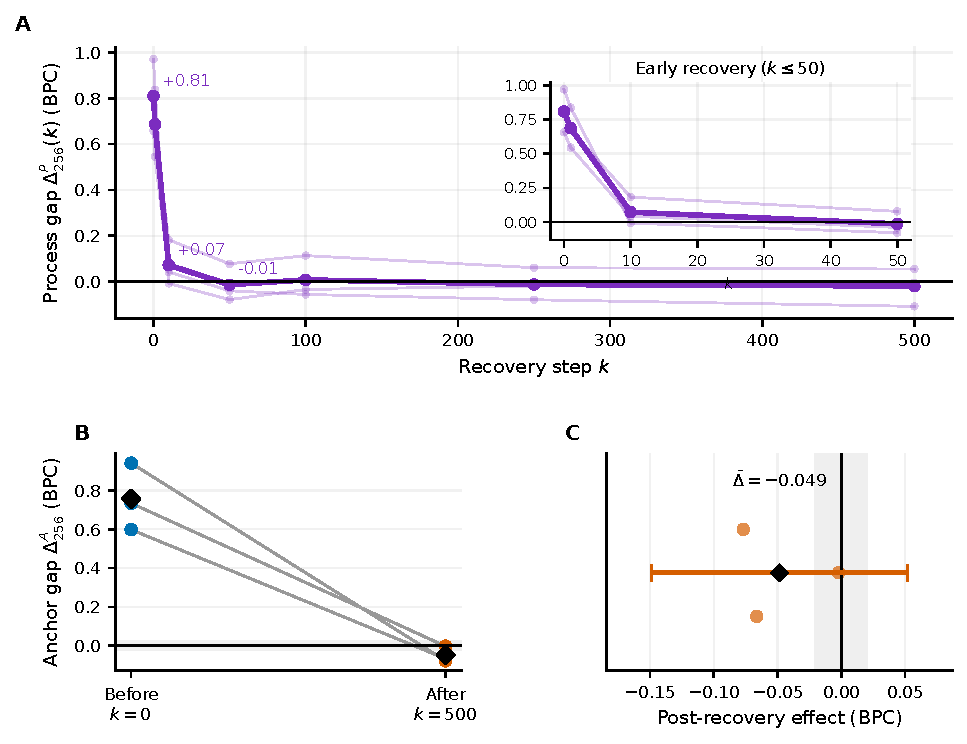
\includegraphics[width=\textwidth]{../../results/recovery_study/figures/paper/v3_r3/main_figure_1_primary_recovery.pdf}
  \caption{\textbf{Common long-context recovery rapidly reverses the large deficit, but the residual is unresolved.} (A) Descending-minus-ascending process-panel BPC at evaluation horizon 256. Pale lines are paired seeds; the heavy line is their mean; markers are measured checkpoints. (B) Anchor-panel contrasts before and after recovery. Lines pair the same seed and do not imply unmeasured dynamics; diamonds are means; gray denotes the preregistered $\pm0.02$ BPC practical-removal region. (C) Seed-level post-recovery effects and the mean with a 95\% Student-$t$ interval. The mean reverses sign, remains outside the removal band, and has an interval crossing zero.}
  \label{fig:primary}
\end{figure*}

The process panel resolves the time scale (Figure~\ref{fig:primary}A). The mean $h=256$ gap falls from $+0.8097$ BPC at $k=0$ to $+0.0719$ at $k=10$ and crosses zero by $k=50$. This rapid change makes a large persistent positive penalty implausible in this setting. It does not establish that all order effects vanish.

\subsection{The initial deficit is horizon-specific}

At step 2000, mean anchor contrasts at horizons 32, 64, 128, and 256 are respectively $-0.0667$, $-0.0424$, $-0.0258$, and $+0.7570$ BPC (Figure~\ref{fig:horizon}). Thus the large deficit is not a uniform deterioration: it appears specifically when the evaluation supplies the long context last used by the ascending arm but not the descending arm. After recovery, all four point estimates are modest and negative ($-0.0622$, $-0.0569$, $-0.0606$, and $-0.0485$), and every three-seed interval crosses zero.

\begin{figure}[t]
  \centering
  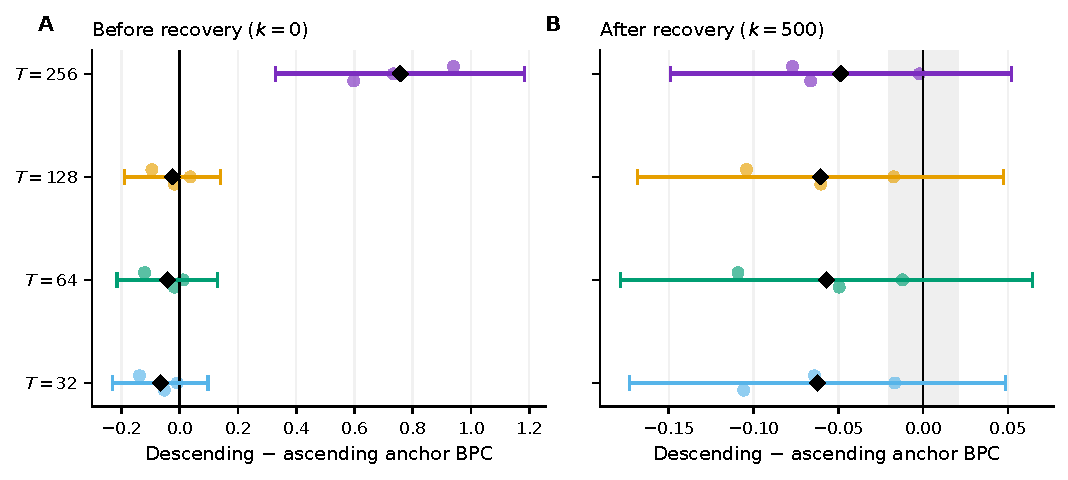
\includegraphics[width=\columnwidth]{../../results/recovery_study/figures/paper/v3_r3/main_figure_2_horizon_specificity.pdf}
  \caption{\textbf{The pre-recovery deficit is specific to long-context evaluation.} Paired seed effects (circles), means (diamonds), and 95\% Student-$t$ intervals before (A) and after (B) common recovery. Panel B includes the preregistered $\pm0.02$ BPC region. Independent horizontal scales expose the smaller post-recovery effects; numeric axes, not bar length, determine magnitude.}
  \label{fig:horizon}
\end{figure}

\subsection{Horizon dependence collapses early in recovery}

The context-alignment contrast $A^P(k)$ falls sharply in the first ten recovery updates and is approximately $0.05$ BPC by step 50 (Figure~\ref{fig:alignment}). This triangulates with the endpoint and multi-horizon results: the original positive gap is strongly coupled to evaluation horizon and recent context exposure. We treat this as supporting evidence for terminal-context sensitivity, not as proof of ``recency bias'' as a unique mechanism.

\begin{figure}[t]
  \centering
  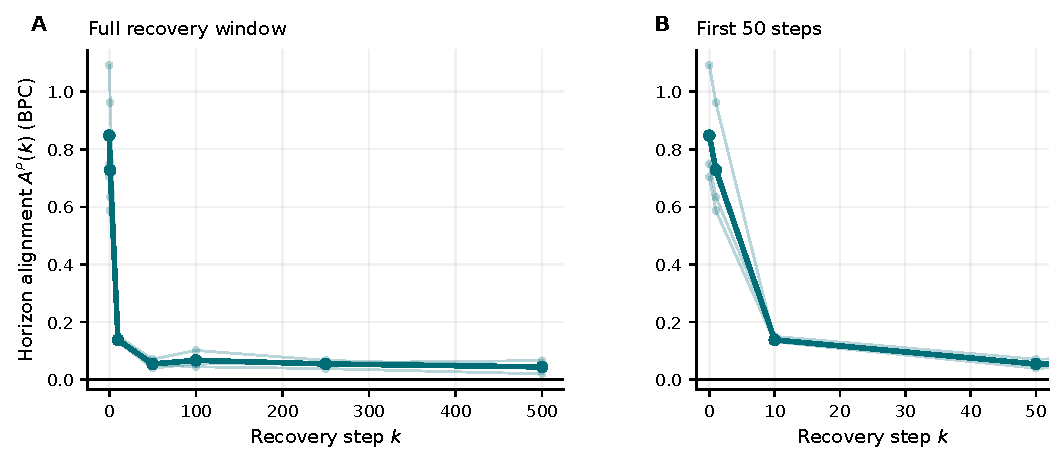
\includegraphics[width=\columnwidth]{../../results/recovery_study/figures/paper/v3_r3/main_figure_3_context_alignment.pdf}
  \caption{\textbf{Most evaluation-horizon dependence disappears within 50 recovery steps.} The process-panel contrast $A^P(k)=\Delta^P_{256}(k)-\Delta^P_{32}(k)$ over the full recovery window (A) and its first 50 steps (B). Pale lines are seeds; heavy lines are means; markers are measured checkpoints. The trajectory supports a terminal-context-sensitive account but does not isolate its mechanism.}
  \label{fig:alignment}
\end{figure}

\section{Discussion}

The experiment changes the interpretation of the terminal gap. Without recovery, one could report that descending order causes a $0.76$ BPC long-context penalty. That statement is true at the endpoint but misleading as a claim about durable path dependence: ten matched long-context updates remove most of the gap, and 50 reverse its sign. Multiple horizons further show that the deficit is conditional on how the model is queried.

The result also demonstrates why no single diagnostic is sufficient. A final anchor panel supplies a higher-precision registered endpoint but hides when recovery occurs. A dense process panel exposes the transition dynamics but uses fewer validation sequences. Multi-horizon evaluation reveals whether the effect is general or context-specific. Pairing reduces irrelevant variance, while raw seeds and intervals prevent the mean trajectory from masquerading as high-powered evidence. Together these measurements answer a sharper question than a larger terminal benchmark alone.

The sign reversal deserves restraint. It is consistent across the three point estimates, but the mean interval crosses zero and the effect misses the preregistered practical-removal band. It may be sampling variation, a smaller path-dependent effect, or an interaction induced by 500 additional long-context updates. The current experiment was designed to decide whether a large \emph{positive} residual justifies mechanism work; that condition was not met. Resolving the negative residual requires more paired seeds or a purpose-built follow-up, not a post hoc redefinition of success.

\section{Limitations}

The study uses one small character-level Transformer, one corpus, one optimizer policy, and three seeds. The results should not be generalized to subword models or large-scale pretraining without replication. Recovery changes both exposure to long context and elapsed optimization time, so the design identifies recovery behavior rather than a unique causal component. Because block order occurs along a fixed global learning-rate trajectory, the estimand includes order-by-training-state interactions. The $0.02$ and $0.03$ BPC thresholds are prespecified project decisions, not field-wide equivalence margins. Finally, one nonmonotonic permutation cannot characterize nonmonotonic curricula as a class.

\section{Conclusion}

A large terminal long-context deficit after descending sequence-length training does not survive common long-context recovery in this experiment. The deficit is horizon-specific and mostly disappears within tens of updates, contradicting a simple persistent-positive-path-dependence account. Yet the endpoint reverses beyond the preregistered practical-removal band, and three seeds cannot resolve that residual. More broadly, sequence-order claims should be supported by a counterfactual recovery stage, transition-local trajectories, and evaluations that vary the context supplied at test time.

\section*{Impact Statement}

This work concerns experimental methodology for language-model training. Better separation of transient and persistent effects may reduce wasted compute and discourage overclaiming from terminal evaluations. The experiments use public-domain text and a small model; we do not identify immediate societal harms beyond the general environmental and reproducibility costs of machine-learning experimentation.

\bibliography{references}
\bibliographystyle{icml2026}

\clearpage
\appendix
\onecolumn

\section{Reproducibility Details}
\label{app:repro}

\begin{table}[h]
\centering
\small
\caption{Frozen model and optimization configuration.}
\begin{tabular}{ll}
\toprule
Component & Value \\
\midrule
Parameters & 4.8M \\
Layers / heads / width & 6 / 8 / 256 \\
Maximum context & 256 characters \\
Position encoding & RoPE \\
Dropout & 0 \\
Optimizer & AdamW \\
Learning rate & $10^{-3}$, minimum $10^{-4}$ \\
Warmup & 400 steps \\
Weight decay / clipping & 0.1 / 1.0 \\
Tokens per update & 4,096 \\
Scheduled / recovery steps & 2,000 / 500 \\
Seeds & 42, 43, 44 \\
Device & Apple M3, 24 GB, MPS \\
\bottomrule
\end{tabular}
\end{table}

Context-specific batch sizes were 128, 64, 32, and 16 for lengths 32, 64, 128, and 256. The process checkpoints were steps 250, 500, 501, 750, 1000, 1001, 1250, 1500, 1501, 1750, 2000, 2001, 2010, 2050, 2100, 2250, and 2500. The preregistration commit was \texttt{f1bf7b7}; training artifacts were produced at \texttt{30a126cb7fbe}; corrected analysis at \texttt{82a4f0d5b24d}; and manuscript figures at \texttt{688d98ad543b}. Full hashes are recorded in the repository technical report.

The runs, estimands, panels, thresholds, and primary rules were frozen before training. Figure hierarchy and styling were designed after inspecting the results. An early post-result analysis treated a sufficiently negative endpoint as practical removal; we reverted it because removal was preregistered by absolute magnitude. No model was retrained and no endpoint was changed.

\section{Complete Multi-Horizon Recovery Trajectories}

\begin{figure}[H]
  \centering
  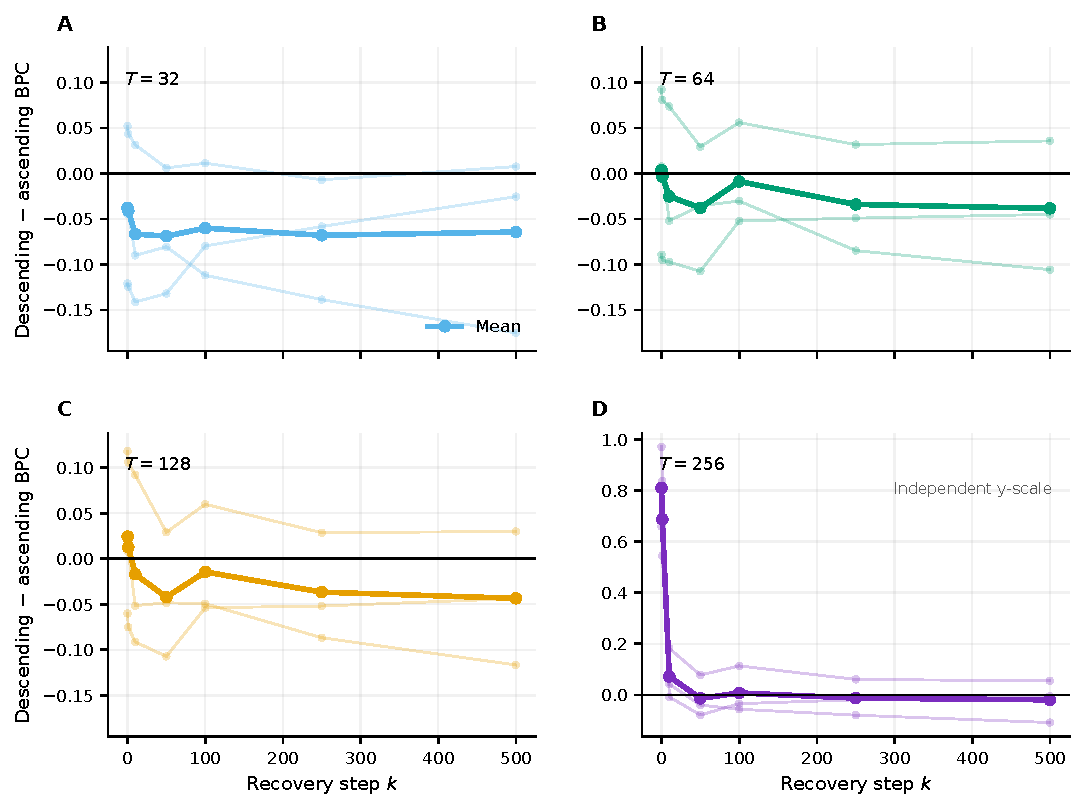
\includegraphics[width=0.82\textwidth]{../../results/recovery_study/figures/paper/v3_r3/appendix_figure_A1_all_horizon_trajectories.pdf}
  \caption{\textbf{Complete recovery trajectories at all evaluation horizons.} Descending-minus-ascending process-panel BPC at every measured recovery checkpoint. Pale lines are paired seeds and heavy lines are means. Panels for horizons 32--128 share a vertical range; the 256-token panel uses a labeled independent range because its initial gap is an order of magnitude larger.}
  \label{fig:allhorizons}
\end{figure}

\section{Exploratory Nonmonotonic Schedule}
\label{app:nonmono}

\begin{figure}[H]
  \centering
  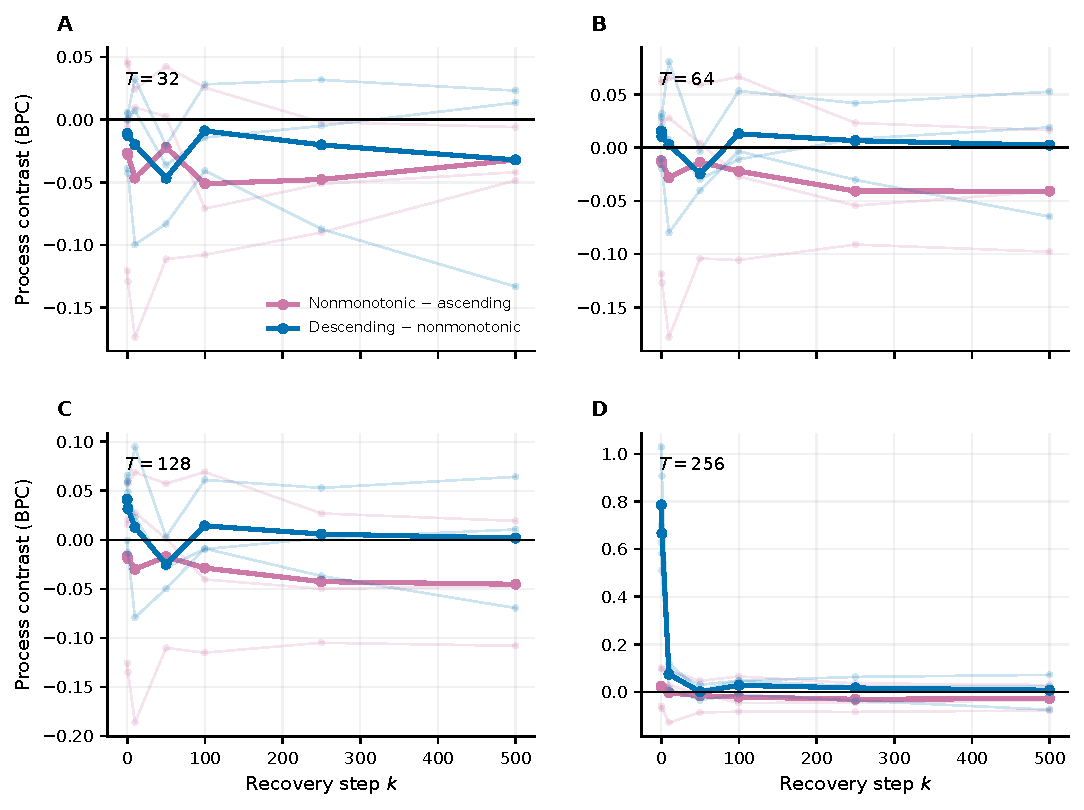
\includegraphics[width=0.82\textwidth]{../../results/recovery_study/figures/paper/v3_r3/appendix_figure_A2_nonmonotonic_exploratory.pdf}
  \caption{\textbf{Exploratory results for one prespecified nonmonotonic permutation.} Pink is nonmonotonic minus ascending; blue is descending minus nonmonotonic; pale lines are seeds and heavy lines are means. The schedule $64{\rightarrow}256{\rightarrow}32{\rightarrow}128$ is one permutation only and does not support claims about nonmonotonic schedules as a class. It does not enter the primary decision.}
  \label{fig:nonmono}
\end{figure}

\section{Seed-Level Primary Results and Decision Logic}

\begin{table}[h]
\centering
\small
\caption{Paired descending-minus-ascending anchor contrasts at horizon 256.}
\begin{tabular}{lrrr}
\toprule
Seed & Pre & Post & Reduction \\
\midrule
42 & 0.5977 & -0.0663 & 0.6640 \\
43 & 0.7336 & -0.0022 & 0.7357 \\
44 & 0.9399 & -0.0770 & 1.0169 \\
\midrule
Mean & 0.7570 & -0.0485 & 0.8055 \\
SD & 0.1723 & 0.0405 & 0.1865 \\
\bottomrule
\end{tabular}
\end{table}

The registered cases were: (A) the initial gap did not replicate, $|\overline{\Delta^A(0)}|<0.02$; (B) practical removal, $|\overline{\Delta^A(500)}|\leq0.02$; (C) a small, directionally inconsistent, or boundary residual; (D) a positive residual above $0.03$ that was still recovering, triggering one extension; and (E) a positive residual above $0.03$, positive in all seeds, and plateaued, justifying a targeted mechanism experiment. The observed negative residual had magnitude $0.0485$ and therefore was not Case B. It also could not satisfy D or E, which were defined for a persistent positive deficit. We record it as Case C rather than moving the threshold after observing the result.

\end{document}
